\documentclass[11pt, a4paper]{article}
\usepackage[paper=a4paper, left=1.5cm, right=1.5cm, bottom=1.5cm, top=1.5cm]{geometry}

\usepackage[utf8]{inputenc}
\usepackage[T1]{fontenc}
\usepackage[spanish]{babel}
\usepackage[section]{placeins}
%\usepackage{csvsimple}
\usepackage{caratula/caratula}
\usepackage{listings}
\usepackage{algpseudocode}
\usepackage{graphicx}
\usepackage{float}
\usepackage{amsmath}
\usepackage{booktabs}
\usepackage[
singlelinecheck=false % <-- important
]{caption}
%\usepackage[spanish,es-noshorthands,es-lcroman]{babel}
%\usepackage{adjustbox}
\usepackage{blindtext}
\usepackage{sidecap}
\usepackage{color}

\usepackage{algorithm}% http://ctan.org/pkg/algorithms
\usepackage{algpseudocode} % Para algorritmia

\begin{document}

\titulo{Trabajo Práctico \#3}
\fecha{17 de Junio de 2014}
\materia{Teoría de las comunicaciones}
% \grupo{Grupo 11}
\integrante{Leandro Matayoshi}{79/11}{leandro.matayoshi@gmail.com}
\integrante{Jonathan Melnik}{571/09}{jonathanmelnik@gmail.com}
\integrante{Martin Santos}{413/11}{martin.n.santos@gmail.com}


%Carátula
\maketitle
\newpage
%Indice
\tableofcontents
\newpage

\section{Introducción}

En este trabajo estudiaremos el transporte de paquetes a través del protocolo PTC proporcionado por la cátedra. Este protocolo está basado en TCP, pero simplificado. Sus características son que es bidireccional(full-duplex), orientado a conexión, y es confiable(usa el algoritmo de ventana deslizante). 

El objetivo del trabajo es estudiar la eficiencia y comportamiento del protocolo al transferir paquetes en una red. Como el trabajo se basará en experimentaciones sobre una red local, la cual no es muy propensa a errores y por ende no se asimila al comportamiento de una red "real", se hizo una implementación de cliente-servidor que permite simular una red "real". Esto es, simulamos los efectos de problemas comunes que existen al transferir paquetes, como son la pérdida de paquetes y la latencia.	

\section{Desarrollo}

Para realizar este trabajo, planteamos distintas formas de simular el comportamiento de una red “real”.
 
Realizamos experimentaciones simulando la latencia, variando el delay en que se envían los ACKs y simulando la perdida de paquetes, mediante una probabilidad arbitraria por que la se decide si enviar un paquete o no. Implementamos un cliente custom, para cada una de las experimentaciones que se comunica con un mismo servidor.

Para crear delay en el envío de los ACKs, modificamos el código proporcionado por la cátedra(protocol.py) e implementamos un timer, de modo que cuando se está por enviar un paquete(usando send\_and\_queue), se chequea si es un ACK, y en ese caso, si el valor del delay es mayor a 0, se usa el timer para llamar a la función que envía el paquete pasado el tiempo igual al valor de delay.

De manera similar, para hacer que los paquetes se pierdan con una cierta probabilidad, en el mismo método, donde agregamos el timer, agregamos una condición que chequee si un un valor random es menor a la chance de perder el paquete. En caso de que lo sea, evitamos llamar a la función send del socket, simulando la pérdida del paquete en el otro punto del canal de comunicación.

En las distintas experimentaciones, variamos el delay de 2 maneras, usando valores constantes y un rango de valores aleatorios. Hicimos lo mismo para el delay. 
La elección de valores constantes o aleatorios en cada experimentación, dependió de lo que se estaba testeando. En los casos en los que el objetivo era testear el comportamiento de la red en función de los valores del del delay o de la perdida de paquetes, usamos valores constantes, para tener control sobre la experimentación y poder explicar los resultados. En caso contrario utilizamos valores aleatorios.

Los valores aleatorios, como dijimos, fueron tomados de un rango de valores posibles. Estos rangos variaron en los distintos experimentos. El rango usado para la probabilidad de perder un paquete fue de 0.98 a 1.00 aproximadamente, o sea de hasta un 2\% de chance de perder un paquete. Para el delay usamos rangos de entre 0.05 y 0.15 segundos. Estos valores fueron calculados a partir de observaciones usando ping a distintos dominios de internet(para el delay) y probando valores que fuesen visibles al realizar las experimentaciones.

Una decisión que tomamos para simular mejor el comportamiento de una red “real” fue hacer que los valores aleatorios para el delay y la chance de perder paquetes varíe constantemente en esos rangos, durante la comunicación entre el cliente y el servidor. La implementación de esta funcionalidad fue usar un thread que llama a una función cada 10 milisegundos y toma un valor aleatorio en el rango posible para las variables. De esta forma, el delay y la probabilidad de pérdida de paquetes resultaron realmente aleatorios en las experimentaciones que lo utilizaron.

Como el trabajo consistía en obtener resultados del comportamiento de la red, lo que hicimos fue enviar archivos entre 2 terminales de la red. Para esto usamos el código proporcionado por la cátedra para crear el canal de comunicación, y sobre este canal creamos un protocolo muy simple para enviar archivos de una terminal a otra. En el protocolo, solo el server recibe archivos y el cliente los envía. El protocolo basa la comunicación en una serie de mensajes definidos como constantes de 10 bytes. Utilizamos mensajes de tamaño constante, ya que la función recv de Socket, recibe como parámetro la cantidad de bytes que va a recibir y hasta que no reciba esa cantidad queda bloqueado, entonces nos aseguramos que intercambiando mensajes de tamaño constante, el servidor y el cliente siempre puedan llamar a recv esperando un mensaje de 10 bytes y así continuar con el intercambio de mensajes. De esta manera, el servidor, comienza escuchando en el socket por un mensaje que puede ser una señal para avisar que se va a mandar un nuevo archivo o que se puede cerrar. Si se va a mandar un nuevo archivo, el servidor contesta al cliente un OK, y el cliente al recibirlo manda el tamaño del archivo que va a mandar, luego espera por otro OK del servidor y comienza mandar el archivo. De esta manera, el servidor sabe con que cantidad de bytes llamar a recv para obtener todo el archivo. Al terminar el servidor queda escuchando nuevamente por un mensaje para recibir otro archivo o cerrarse.

\section{Resultados y análisis}

\subsection{Throughput percibido en funcion del tamaño de archivo}

En esta sección vamos a analizar la velocidad de tranmisión de diversos archivos a través de una red local utilizando el protocolo PTC. Para ello montamos un server en determinada máquina, llamémosla A y, un cliente, B, en otra máquina de la misma red. Antes de poder comenzar el envío de datos es necesario que tanto A como B establezcan una conexión entre si. Esto se realiza a través de un algoritmo $three-way \ handshake$ implementando en PTC. Una vez establecida la conexión, B envía varios archivos de distintos tamaños y, por cada archivo, calcula el tiempo insumido en realizar dicha acción para luego calcular el $throughput$. En definitiva, lo que hacemos es setear un timer que arranca cuando se comienza a enviar un archivo desde B y se detiene cuando A le informa que llegó satisfactoriamente. Luego, dividimos el tamaño del archivo enviado (en Bytes) por el tiempo insumido (s) y lo multiplicamos por 1024 para obtener la velocidad en Kb/s.

Analizaremos el $throughput$ percibido en función del tamaño de los archivos enviados testeándolo en diversos entornos. Tomaremos cuatro tipos de entorno posibles:
\begin{itemize}
	\item[1] Entorno sin delay agregado en los ACK's y con probabilidad 0 de que se pierdan paquetes.
	\item[2] Entorno con delay agregado que se va modificando dinámicamente entre 20ms y 80ms con probabilidad 0 de pérdida de paquetes.
	\item[3] Entorno con delay agregado que se va modificando dinámicamente entre 20ms y 80ms con probabilidad 0.05 de pérdida de paquetes.
\end{itemize}

A continuación, los resultados:

\begin{figure}[H]
	\begin{center}
		  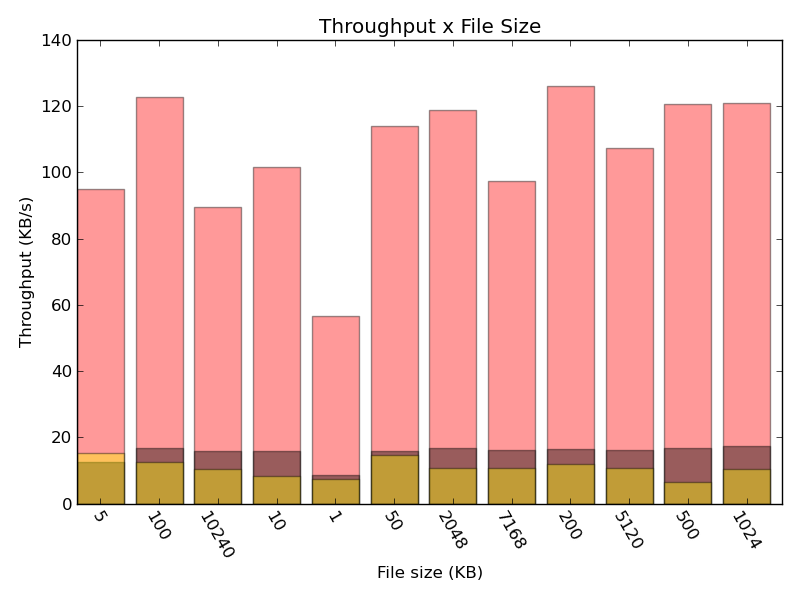
\includegraphics[scale=0.5]{../graficos/test1_1.png}
		  \caption{$Throughput$ en cada entorno en función del tamaño del archivo}
		  \label{fig:contra1}
	\end{center}
\end{figure}

Viendo los resultados obtenidos concluimos en que mientras más 'real' es el entorno peor es el $throughput$ percibido y esto es algo que intuitivamente se esperaba. Si transferimos archivos en un entorno sin delay cuya pérdida de paquetes tiene probabilidad 0 es esperable que tenga una velocidad mucho mayor que en una donde si hay delay y pérdida de paquetes. Esto se ve claramente entre el entorno 1 y 2 y el entorno 1 y 3. La diferencia no es tan grande entre los entornos 2 y 3, en donde la única diferencia es la probabilidad de pérdida de paquetes.

Otro punto a analizar es el $throughput$ en función del tamaño del archivo para cada entorno. Si bien hay diferencia en la velocidad de transmisión para cada archivo esta se mantiene bastante parecida entre todos ellos. El único $throughput$ que difiere bastante es el del archivo de 1KB. Sin embargo debemos tener en cuenta de que se trata de un archivo muy pequeño y cuyo tamaño es igual al del Receive Buffer Size. Por este motivo no debemos darle tanta importancia a ese valor.




\input{resultados.tex}

\section{Conclusiones}

Luego de desarrollar los experimentos a lo largo del trabajo práctico pudimos observar algunos de los problemas con los que debe lidiar el protocolo para ofrecer un servicio confiable a sus usuarios. La pérdida de paquetes y el delay en la entrega de los ACK's son algunas cosas a las que TCP y PTC deben enfrentarse todo el tiempo para lograr tal fin ya que el protocolo IP no incluye ningún monitoreo de la entrega de datagramas. Analizando el Throughput percibido (i.e., cantidad de bits por segundo) en función del tamaño de archivo, Throughput en función del delay en los ACKs (para un tamaño de archivo constante) y la cantidad de retransmisiones en función del delay en los ACKs (para un tamaño de archivo constante) observamos cómo el delay de los ACK's influye negativamente en la velocidad de transmisión. A su vez, este delay y la pérdida de paquetes generan un aumento de retransmisión de paquetes lo cual disminuye aún más la velocidad de transmision pero que asegura una entrega confiable de la información que es el principal objetivo de este protocolo.



\newpage

\section{Apéndice}

\input{apendice.tex}


\end{document}
